%========================================================================
\section{Discovery pour GTT}
% TIMING ~7 min  |  SOMMET D'AUTONOMIE (solo, 1 mois) + FOCUS DIFFICULTES. 2e demarche, en mode discovery.
%========================================================================

% --- S1 : Contexte GTT -------------------------------------------------
\begin{frame}{GTT et la LNG Digital Factory}
  % VOIX ~1 min. Qui est GTT, pourquoi le digital, l'echeance.
  \begin{columns}[T]
    \column{.52\textwidth}
    \begin{itemize}\footnotesize
      \item GTT : leader mondial des systèmes de confinement à membrane pour méthaniers \textbf{(brevet de cuves GNL)}
      \item Volonté de se diversifier vers le digital
      \item Programme \textbf{LNG Digital Factory} : concevoir une solution digitale qui s'impose leader sur le marché du GNL
    \end{itemize}
    \column{.4\textwidth}
    \begin{alertblock}{L'échéance}
      \footnotesize Présentation d'un MVP de la solution à \textbf{Gastech, le 14 septembre}.
    \end{alertblock}
  \end{columns}
\end{frame}

% --- S2 : Ma mission ---------------------------------------------------
\begin{frame}{Benchmarker tout un marché digital}
  % VOIX ~1 min. La contrainte brute.
  \begin{itemize}\footnotesize
    \item Benchmarker l'intégralité de la \textbf{concurrence digitale du secteur GNL}
    \item En un mois, à partir de presque rien (interviews utilisateurs)
    \item Domaine inconnu au départ : jargon maritime, spécificité et contraites du secteur GNL
  \end{itemize}
  \vskip 6pt
  \begin{block}{L'objectif réel}
    \footnotesize Produire non pas un catalogue, mais une cartographie utilisable : Que fait le marché ? Où GTT peut se positionner ? Comment se différencier via cette nouvelle solution digitale ?
  \end{block}
\end{frame}

% --- S3 : La methode ---------------------------------------------------
\begin{frame}{Récupérer le maximum d'informations et la structurer}
  % VOIX ~1 min 30. Le pipeline.
  \begin{itemize}\footnotesize
    \item Collecter : Google Gemini \textbf{Deep Research} pour chaque solution digitale, centralisées dans un NotebookLM
    \item Vérifier : Relecture des Deep Research en \textbf{challengeant} les sources et les informations
    \item Formater : Fiche pour chaque solution digitale (identité, business model, architecture, deep-dive fonctionnel, voix du client, \dots)
    \item Structurer : regroupement en \textbf{7 catégories de solutions} (routage, chantiers navals, \dots)
  \end{itemize}
  \vskip 16pt
  \begin{alertblock}{Résultat}
    \footnotesize $\Rightarrow$ \textbf{23 solutions analysées} de bout en bout et présentées
  \end{alertblock}
\end{frame}

% --- S4 : Screenshot fiche BOSS ---------------------------------------
\begin{frame}[plain]
  % VOIX ~45 s. Montrer le format standardise.
  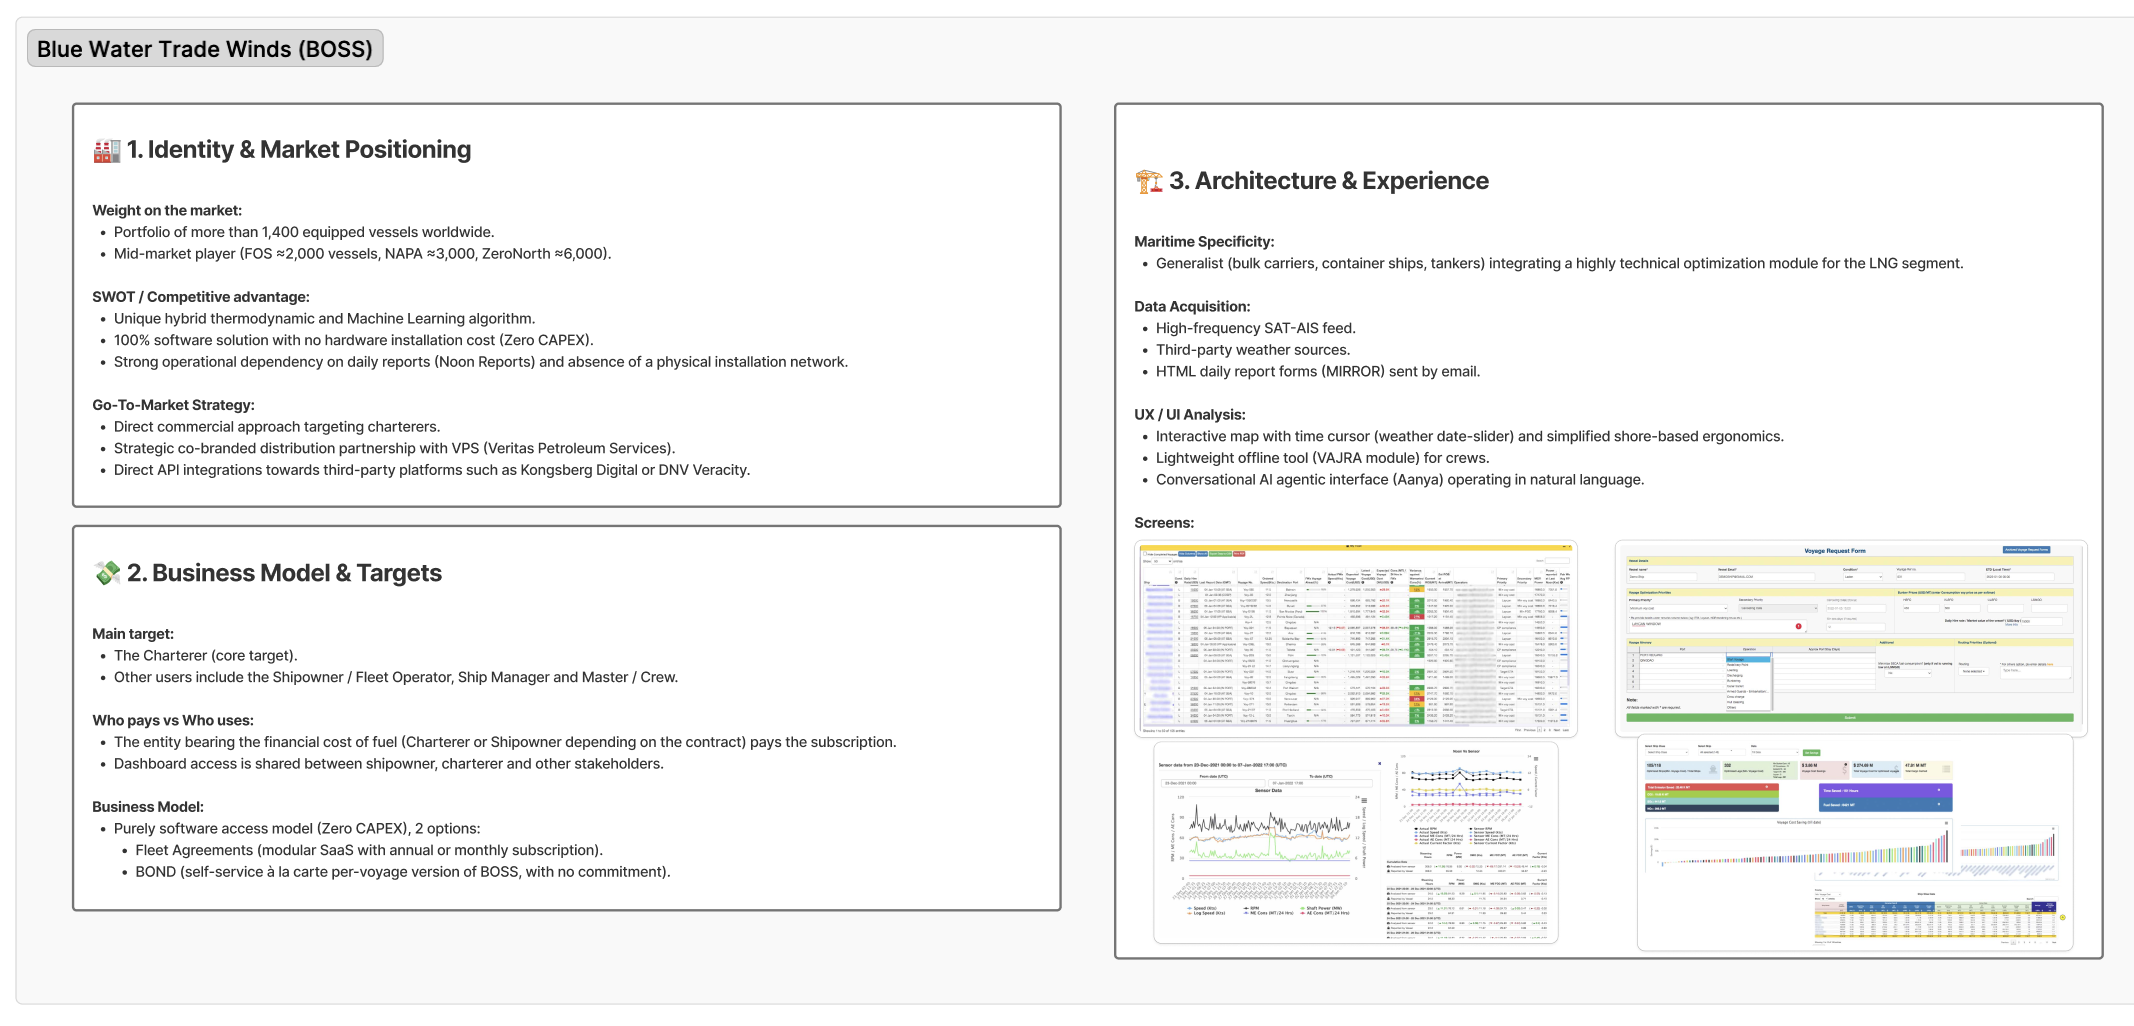
\includegraphics[height=0.8\paperheight,width=\paperwidth,keepaspectratio]{images/figjam_boss_1}
\end{frame}

\begin{frame}[plain]
  % VOIX ~45 s. Repond directement a l'obstacle "confiance dans l'IA".
  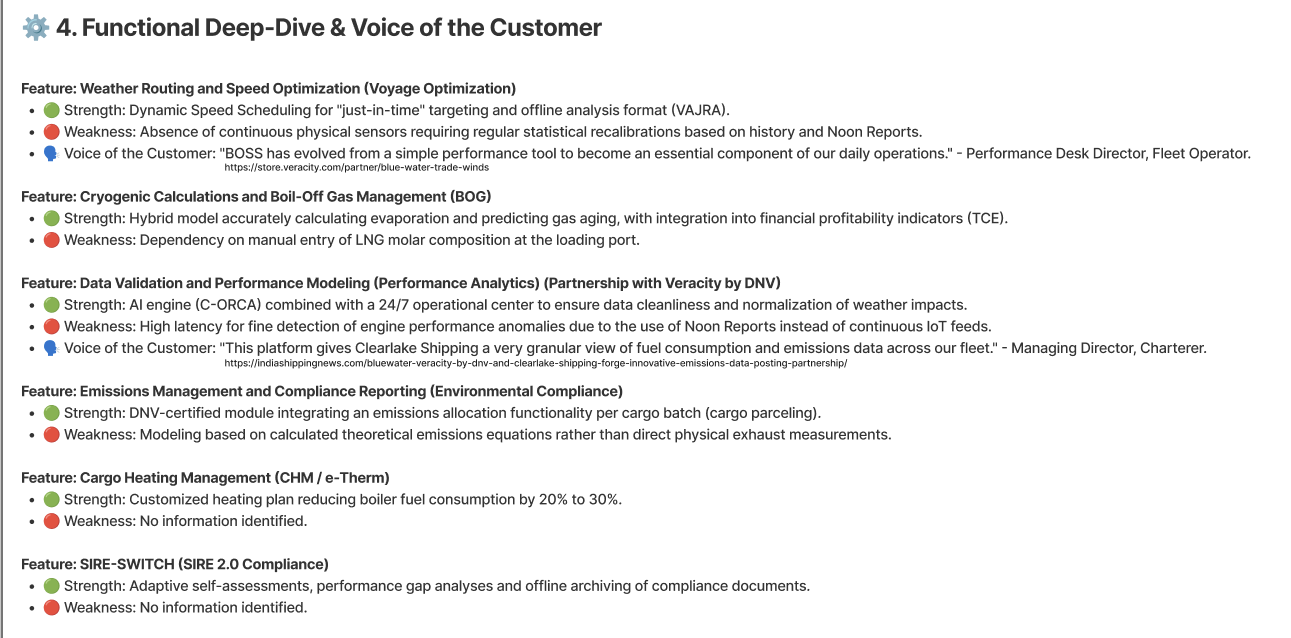
\includegraphics[height=0.8\paperheight,width=\paperwidth,keepaspectratio]{images/figjam_boss_2}
\end{frame}

% --- S6 : Difficultes / reponses --------------------------------------
\begin{frame}{Difficultés de cette approche}
  % VOIX ~2 min. CŒUR de la partie.
  \footnotesize
  \begin{alertblock}{Informations rares liées au monde B2B GNL}
    Réponse : Deep Research combiné à des recherches personnelles (documentation technique, captures d'écrans)
  \end{alertblock}
  \begin{alertblock}{Faire confiance aux sorties du LLM}
    Réponse : itérations sur les informations importantes, vérifications des sources fournies par le Deep Research.
  \end{alertblock}
  \begin{alertblock}{Une masse brute à rendre lisible}
    Réponse : création d'un tableau de synthèse fonctionnalités/solutions digitales.
  \end{alertblock}
\end{frame}

% --- S7 : Screenshot tableau de synthese ------------------------------
\begin{frame}{Le livrable : un tableau de synthèse comparatif}
  % VOIX ~1 min. La matrice fonctionnalites x concurrents.
  \centering
  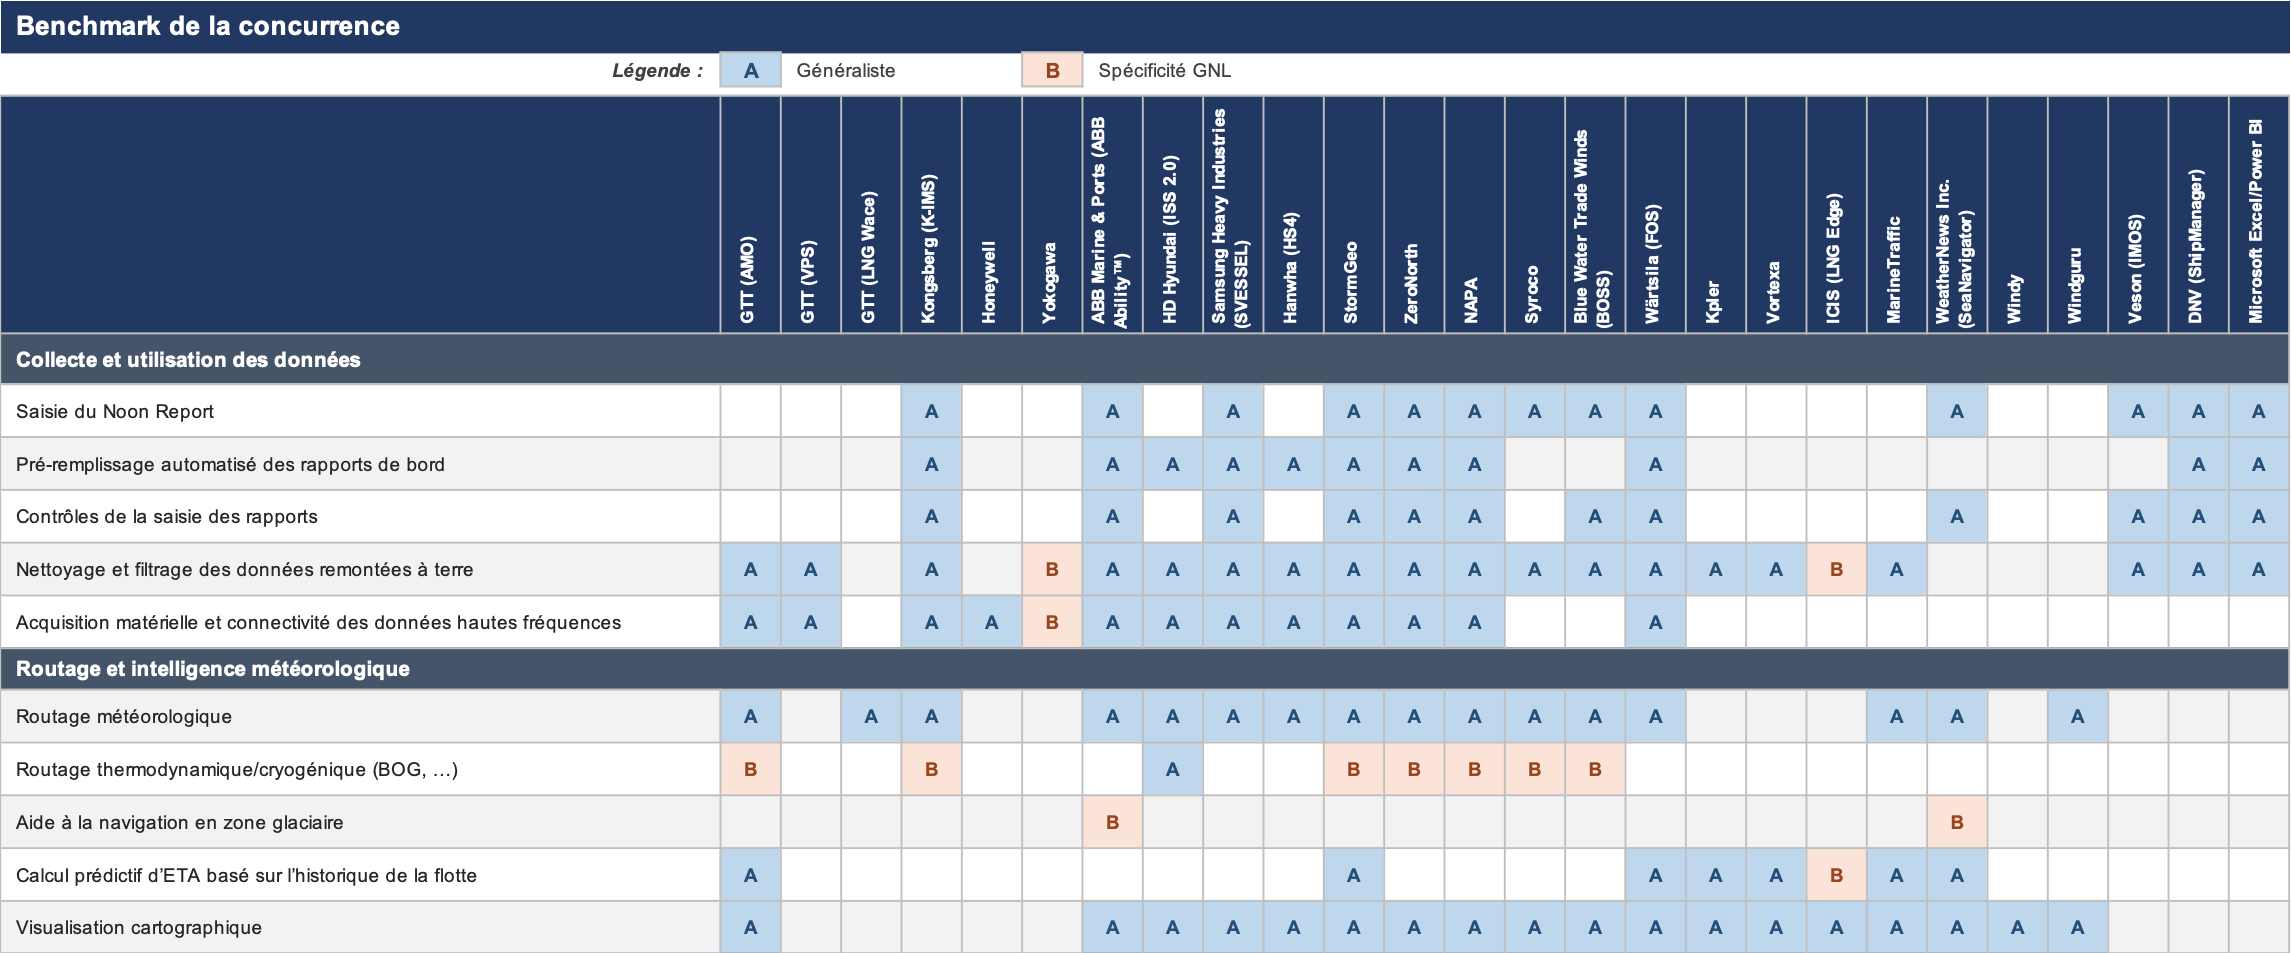
\includegraphics[width=\textwidth]{images/competitive_benchmark_extract.png}\\[3pt]
  {\scriptsize Extrait du tableau fonctionnalités $\times$ concurrents, exploitable en atelier}
\end{frame}

% --- S8 : Limites ------------------------------------------------------
\begin{frame}{Limites de la démarche et pistes de poursuite}
  % VOIX ~1 min 15. Lucidite sur la methode.
  \begin{columns}[T]
    \column{.5\textwidth}
    \begin{alertblock}{Limites}
      \footnotesize
      \begin{itemize}\scriptsize
        \item Basé sur des sources internet, des communications officielles et retours utilisateurs
        \item Benchmark valable à l'instant T
        \item Difficile de pousser plus loin sans avoir accès aux logiciels
      \end{itemize}
    \end{alertblock}
    \column{.45\textwidth}
    \begin{exampleblock}{Pour poursuivre}
      \footnotesize
      \begin{itemize}\scriptsize
        \item Démos produit et interviews directes
        \item Vérifier les informations avec des experts
        \item Mise à jour périodique du benchmark
      \end{itemize}
    \end{exampleblock}
  \end{columns}
\end{frame}

% --- S9 : Conclusion / valeur -----------------------------------------
\begin{frame}{Un benchmark qui oriente la conception}
  % VOIX ~1 min. Le benchmark sert l'action.
  \begin{itemize}\footnotesize
    \item Un outil qui peut continuer d'évoluer en interne chez GTT
    \item En atelier avec GTT : pour chaque fonctionnalité identifiée comme "importante" un arbitrage est possible
    \item Support : NotebookLM complet (Deep Research + documentations techniques) interrogeable et tableau de synthèse
  \end{itemize}
  \vskip 6pt
  \begin{block}{Pour conclure}
    \footnotesize Le benchmark situe GTT face au marché et cadre les choix produit en vue de Gastech.
  \end{block}
\end{frame}
